\documentclass{article}
\usepackage{amssymb}
\usepackage{tikz}
\usepackage[margin=4cm]{geometry}

\title{Modelos Discretos: Respuestas tarea 1}
\author{Francisco Carvajal, Vicente Díaz, Benjamín Farías}

\begin{document}
\maketitle



\section{Inducción Estructural}

\section{Inducción sobre strings}

\section{Definición inductiva de grafos}
%Pancho Tarea

\subsection{Mediante inducción estructural defina la estructura del grafo.}
Debemos definir un grafo de a traves de la induccion estructural, en base a las 
instrucciones se usara una lista de adyacencia, por lo tanto lo primero que 
debemos crear es una lista de numeros para que posteriormente el grafo sea 
una lista de listas de numeros. 
Se define la lista y algunas funciones utiles.

\subsubsection*{\emph{Lista de naturales}}
Definición:
\[ \emptyset \in \mathcal{L}_{\mathbb{N}} \]
\[ L \in \mathcal{L}_\mathbb{N} \Rightarrow L \rightarrow k \in \mathcal{L}_\mathbb{N}, \forall k \in \mathbb{N}\]
Operaciones:
\[ Insertar(L, k) = L \rightarrow k\]


Ejemplos:

\[ \rightarrow 0 \rightarrow 2 \rightarrow 7 \]
\[ Insertar(\rightarrow 0 \rightarrow 2 \rightarrow 7, 10) =  \rightarrow 0 \rightarrow 2 \rightarrow 7 \rightarrow 10\]
\[ Insertar(\emptyset, 4) = \rightarrow 4 \]

\subsubsection*{\emph{Grafo (Direccional)}}
Ahora se crea el grafo utilizando la lista, es importante notar que la definicion 
de este grafo, es la implementacion de un grafo direccional, las listas 
de adyacencia por lo general son para grafos dirigidos. Haremos que sea un grafo
no dirigido posteriormente con el metodo de $InsertarNodo$, ya que, ese metodo creara 
una conexion de i a j y de j a i, manteniendo las propiedades de un grafo no dirigido
\footnote{A excepcion de que en este grafo la cantidad flechas sera el doble que la 
cantidad de aristas reales en el grafo.}. Se utilizara una flecha diferente a la 
de la lista para distingirlas.

Definición:

\[ \emptyset \in \mathcal{G} \]
\[ G \in \mathcal{G} \Rightarrow G \rightarrowtail (l) \in \mathcal{G} , \forall l \in \mathcal{L}_\mathbb{N} \]

Ejemplos:

\[ \rightarrowtail ( \rightarrow 2 \rightarrow 3) \rightarrowtail (\rightarrow 3) \rightarrowtail (\rightarrow 0) \rightarrowtail (\rightarrow 0 \rightarrow 1) \]
representa el siguiente grafo: 

\begin{center}
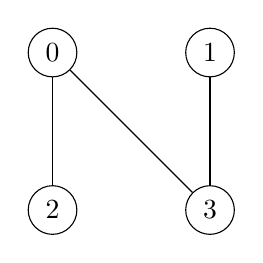
\begin{tikzpicture}
  % Nodos
  \node[circle, draw] (0) at (0,0) {0};
  \node[circle, draw] (1) at (2,0) {1};
  \node[circle, draw] (2) at (0,-2) {2};
  \node[circle, draw] (3) at (2,-2) {3};
  
  % Aristas
  \draw (0) -- (2);
  \draw (0) -- (3);
  \draw (1) -- (3);
\end{tikzpicture}
\end{center}

\subsection{Insertar Nodo}
Esta parte se complica un poco, al ser un grafo no dirigido, ya que, no se puede
solo añadir la lista al final del grafo que ya tenemos, porque se crearia 
asimetria en los datos del grafo, es decir, se puede llegar de j a i, pero 
no de i a j.
Por lo tanto lo que debemos hacer es añadir la lista al final pero ademas 
debemos agregar en cada lista del grafo que corresponda, un borde a la nueva 
arista.
Para hacer esto lo primero que hare es una funcion que conecte el nodo i y j
de un grafo G.

\[ Conectar((L) \rightarrowtail G, 0, j) = (Insertar(L, j)) \rightarrowtail G \]
\[ Conectar((L) \rightarrowtail G, i, j) = (L) \rightarrowtail Conectar(G, i-1, j) \]

Ademas ahora seria util una funcion que conecte una lista de nodos a un nodo,
para utilizarla en la funcion final.

\[ ConectarTodos(G, \emptyset, j) = G  \]
\[ ConectarTodos(G, i \rightarrow L, j) = ConectarTodos(Conectar(G, i, j), L, j)  \]

Ahora que ya podemos conectar el nodo i con el j, necesitamos saber que valor 
tendra j, por lo tanto, tenemos que saber cuantos nodos hay en el grafo para 
conocer cual sera el valor del siguiente.

\[ ContarNodos(\emptyset) = 0 \]
\[ ContarNodos((L) \rightarrowtail G) = 1 + ContarNodos(G) \]

Con estas funciones auxiliares creadas, el trabajo se facilita mucho y ya 
podemos definir la funcion InsertarNodo.

\[ InsertarNodo(G, L) = ConectarTodos(G \rightarrowtail (L), L, ContarNodos(G)) \]

\subsection{Cantidad minima de aristas}

Debemos demostrar $ a_n = n - 1 $ donde $ a_n $ es la minima cantidad de aristas
necesarias para conectar n nodos.

\emph{B.I.}
\[ n = 1 \]

\begin{center}
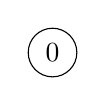
\begin{tikzpicture}
  % Nodos
  \node[circle, draw] (0) at (0,0) {0};
\end{tikzpicture}
\end{center}
En este caso hay 0 aristas, lo que concuerda con $a_1 = 1 - 1 = 0$. :)

\[ n = 2 \]

\begin{center}
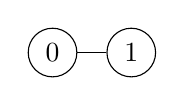
\begin{tikzpicture}
  % Nodos
  \node[circle, draw] (0) {0};
  \node[circle, draw] (1) [right of=0] {1};

  \draw (0) -- (1);
\end{tikzpicture}
\end{center}
En este caso hay 1 arista, lo que concuerda con $a_2 = 2 - 1 = 1$. :)


\[ n = 5 \]

\begin{center}
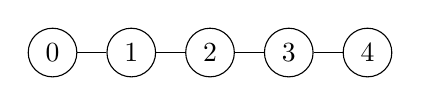
\begin{tikzpicture}
  % Nodos
  \node[circle, draw] (0) {0};
  \node[circle, draw] (1) [right of=0] {1};
  \node[circle, draw] (2) [right of=1] {2};
  \node[circle, draw] (3) [right of=2] {3};
  \node[circle, draw] (4) [right of=3] {4};

  \draw (0) -- (1);
  \draw (2) -- (1);
  \draw (2) -- (3);
  \draw (4) -- (3);
\end{tikzpicture}
\end{center}
En este caso hay 4 aristas, lo que concuerda con $a_5 = 5 - 1 = 4$. :)

\emph{H.I.}
Ahora vamos asumir que $ a_n = n - 1 $.

\emph{T.I.}\\
PDQ: $a_{n+1} = (n + 1) -1 = n$ \\
Si tenemos un grafo que ya esta minimamente conectado y queremos añadir un nodo
tenemos que añadir solo una arista para conectar ese nodo, y mantenemos el estado minimo 
del grafo. Es decir:

\[a_{n+1} = a_{n} + 1\]
Por H.I
\[a_{n+1} = (n - 1) + 1\]
\[a_{n+1} = n\]
 

\subsection{Cantidad maxima de aristas}
Demos demostrar $a_n = \frac{n(n-1)}{2} $ donde $a_n$ es la maxima cantidad de 
aristas que podemos utilizar para conectar n nodos.

\subsubsection*{\emph{B.I}}
\[ n = 1 \]

\begin{center}
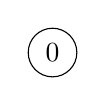
\begin{tikzpicture}
  % Nodos
  \node[circle, draw] (0) at (0,0) {0};
\end{tikzpicture}
\end{center}
En este caso hay 0 aristas, lo que concuerda con $a_1 = \frac{1(1-1)}{2} = 0$. :)

\[ n = 2 \]

\begin{center}
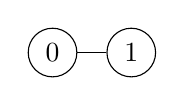
\begin{tikzpicture}
  % Nodos
  \node[circle, draw] (0) {0};
  \node[circle, draw] (1) [right of=0] {1};

  \draw (0) -- (1);
\end{tikzpicture}
\end{center}
En este caso hay 1 arista, lo que concuerda con $a_2 = \frac{2(2-1)}{2} = 1$. :)


\[ n = 5 \]

\begin{center}
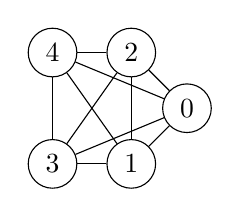
\begin{tikzpicture}
  % Nodos
  \node[circle, draw] (0) {0};
  \node[circle, draw] (1) [below left of=0] {1};
  \node[circle, draw] (2) [above left of=0] {2};
  \node[circle, draw] (3) [left of=1] {3};
  \node[circle, draw] (4) [left of=2] {4};

  \draw (0) -- (1);
  \draw (0) -- (2);
  \draw (0) -- (3);
  \draw (0) -- (4);
  \draw (1) -- (2);
  \draw (1) -- (3);
  \draw (1) -- (4);
  \draw (2) -- (3);
  \draw (2) -- (4);
  \draw (3) -- (4);
\end{tikzpicture}
\end{center}
En este caso hay 10 aristas, lo que concuerda con $a_5 = \frac{5(5-1)}{2}$ = 10. :)

\subsubsection*{\emph{H.I}}
Ahora asumiremos correcto que:
\[ a_n = \frac{n(n-1)}{2} \]

\subsubsection*{\emph{T.I}}
\emph{PDQ:}
\[ a_{n+1} = \frac{(n+1)((n+1) - 1)}{2} = \frac{(n+1)n}{2} \]
Si tenemos un grafo que esta maximamente conectado con n nodos y queremos añadir
uno nuevo, podemos añadir como maximo n aristas, ya que, sera añadida una conexion a 
cada nodo que ya estaba en el grafo, no podemos añadir mas debido todas las otras 
ya estan en el grafo por estar maximamente conectado.
\[ \therefore a_{n+1} = a_n + n \]
\emph{Por H.I.}
\[ a_{n+1} = \frac{(n-1)n}{2} + n = \frac{(n-1)n + 2n}{2} = \frac{n(n-1+2)}{2} = \frac{(n+1)n}{2} \]


\section{Inducción para resolver sumatorias}

\section{Inducción sobre fórmulas lógicas}

\section{Inducción sobre números naturales}

\section{Falacias inductivas}

\end{document}
